\documentclass[5p,12pt]{elsarticle}
\usepackage{amsmath}
\usepackage{amssymb}
\usepackage{xcolor}
\usepackage{tikz}

\newcommand{\pr}[1]{p_{#1}}

\newcommand{\temp}[1]{T_{#1}}

\newcommand{\Nodes}{V}

\newcommand{\Edges}{E}

\newcommand{\mf}[1]{\dot{m}_{#1}}

\newcommand{\tempstart}[1]{\temp{#1}^{start}}

\newcommand{\tempend}[1]{\temp{#1}^{end}}

\begin{document}

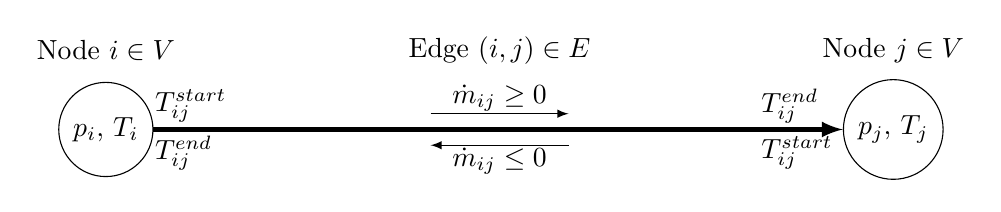
\begin{tikzpicture}
    % Nodes and Edge: 
    \node at ( 0, 3) [circle, draw] (01) {$\pr{i}$, $\temp{i}$};
    \node at (10, 3) [circle, draw] (02) {$\pr{j}$, $\temp{j}$};
    \draw[ultra thick, -latex] (01) -- (02);
    % text on top: 
    \node[] at ( 0, 4) {Node $i \in \Nodes$};
    \node[] at (10, 4) {Node $j \in \Nodes$};
    \node[] at ( 5, 4) {Edge $(i,j) \in \Edges$};
    % top mf: 
    \node at (4,3.2) (tl) {}; 
    \node at (6,3.2) (tr) {};
    \draw[-latex] (tl) -- (tr);
    \node at (5, 3.4) (t) {$\mf{ij} \geq 0$};
    % top Tend / Tstart
    \node[anchor=west] at (0.5, 3.3) {$\tempstart{ij}$};
    \node[anchor=west] at (8.2, 3.3) {$\tempend{ij}$};
    % bottom mf: 
    \node at (4,2.8) (bl) {}; 
    \node at (6,2.8) (br) {};
    \draw[-latex] (br) -- (bl);
    \node at (5, 2.6) (b) {$\mf{ij} \leq 0$};
    % top Tend 
    \node[anchor=west] at (0.5, 2.7) {$\tempend{ij}$};
    \node[anchor=west] at (8.2, 2.7) {$\tempstart{ij}$};

\end{tikzpicture}

\end{document}